\vspace{1em}
\scalebox{0.85}{
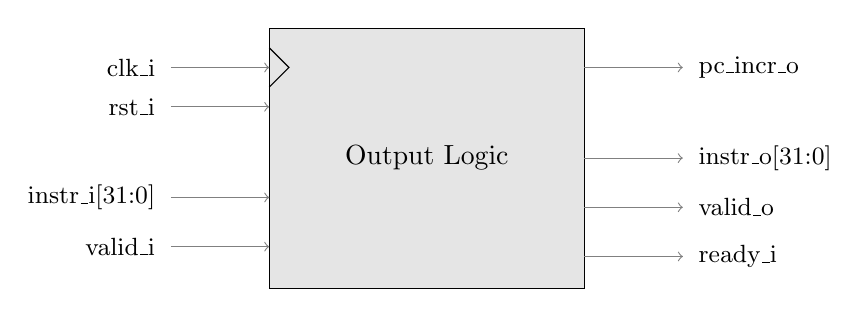
\begin{tikzpicture}[scale=1.25, draw=gray, inner sep=0, outer sep=0]
  \node[rectangle, draw=black,
    anchor=south,
    align=center,
    minimum height = 3.3cm,
    minimum width = 4cm,
    fill = gray!20] (block) at (0, 0) {Output Logic};

  \node(lport1) at ([yshift=-0.4cm]block.west) {};
  \node(lport2) at ([yshift=-0.5cm]lport1.center) {};
  \draw[->] ([xshift=-1cm]lport1.center) node[left=0.2cm, anchor=east]{\small instr\_i[31:0]} -- (lport1.center);
  \draw[->] ([xshift=-1cm]lport2.center) node[left=0.2cm, anchor=east]{\small valid\_i} -- (lport2.center);

  \node(rport1) at ([yshift=-0.4cm]block.north east) {};
  \node(rport2) at (block.east) {};
  \node(rport3) at ([yshift=-0.5cm]rport2.center) {};
  \node(rport4) at ([yshift=-0.5cm]rport3.center) {};
  \draw[<-] ([xshift=1cm]rport1.center) node[right=0.2cm, anchor=west]{\small pc\_incr\_o} -- (rport1.center);
  \draw[<-] ([xshift=1cm]rport2.center) node[right=0.2cm, anchor=west]{\small instr\_o[31:0]} -- (rport2.center);
  \draw[<-] ([xshift=1cm]rport3.center) node[right=0.2cm, anchor=west]{\small valid\_o} -- (rport3.center);
  \draw[<-] ([xshift=1cm]rport4.center) node[right=0.2cm, anchor=west]{\small ready\_i} -- (rport4.center);

%  \node(uport4) at ([xshift=0.5cm]block.north) {};
%  \node(uport3) at ([xshift=-0.5cm]uport4.center) {};
%  \node(uport2) at ([xshift=-0.5cm]uport3.center) {};
%  \node(uport1) at ([xshift=-0.5cm]uport2.north) {};
%  \node(uport5) at ([xshift=0.5cm]uport4.center) {};
%  \draw[<-] ([yshift=1cm]uport1.center) node[above=0.2cm, anchor=west, rotate=45]{\small wb\_clk\_o} -- (uport1.center);
%  \draw[<-] ([yshift=1cm]uport2.center) node[above=0.2cm, anchor=west, rotate=45]{\small wb\_adr\_o[31:0]} -- (uport2.center);
%  \draw[->] ([yshift=1cm]uport3.center) node[above=0.2cm, anchor=west, rotate=45]{\small wb\_dat\_i[31:0]} -- (uport3.center);
%  \draw[<-] ([yshift=1cm]uport4.center) node[above=0.2cm, anchor=west, rotate=45]{\small wb\_stb\_o} -- (uport4.center);
%  \draw[->] ([yshift=1cm]uport5.center) node[above=0.2cm, anchor=west, rotate=45]{\small wb\_ack\_i} -- (uport5.center);
%
%
%  \node(rport2) at ([yshift=-0.5cm]rport1.center) {};
%  \draw[<-] ([xshift=1cm]rport2.center) node[right=0.2cm, anchor=west]{\small valid\_o} -- (rport2.center);
%
  \node (clk) at ([yshift=-0.4cm]block.north west) {};
  \draw[->] ([xshift=-1cm]clk.center) node[left=0.2cm, anchor=east]{\small clk\_i} -- (clk.center);
  % clk triangle
  \draw[-, draw=black] ([yshift=0.2cm]clk.center) -- ([xshift=0.2cm]clk.center) -- ([yshift=-0.2cm]clk.center);

  \node (rst) at ([yshift=-0.4cm]clk.center) {};
  \draw[->] ([xshift=-1cm]rst.center) node[left=0.2cm, anchor=east]{\small rst\_i} -- (rst.center);
\end{tikzpicture}
}
